\chapter{Desarrollo de prototipos}
\label{cap:Desarrollo de prototipos}

El capítulo actual tiene como objetivo presentar en orden temporal los distintos prototipos que se han desarrollado hasta llegar a la versión final que se presenta en el capítulo \ref{cap:ChatBot final}. 

La estructura del capítulo  muestra en orden lineal en el tiempo como se ha ido construyendo la arquitectura del sistema. De esta forma se puede ver como el modelo va pasando por distintos prototipos de forma incremental. 

En este capítulo, también se pretende mostrar y hacer hincapié en los diferentes desafíos, contratiempos y retos a los que ha habido que hacer frente durante el desarrollo del prototipo, por qué se han originado y cómo se han solucionado. 

Con todo ello, se pretende tener una visión global de lo que ha sido el trabajo de desarrollo del sistema. Partiendo de la situación que se muestra en el capítulo \ref{cap:estadoDeLaCuestion}, y teniendo en cuenta el estudio teórico llevado a cabo en el capítulo \ref{cap:introduccion} se trata de hacer un chatbot que facilite tanto como sea posible las tareas de extracción de la información en la terapia de reminiscencia. Para ello se usan las distintas herramientas detalladas en el capítulo \ref{cap:TecnologiasUtilizadas} dando lugar al sistema que se presentará en el capítulo \ref{cap:ChatBot final} \footnote{El repositorio con el código se puede consultar en \href{ GitHub}{github:\\
		https://github.com/NILGroup/TFG-2324-ChatbotCANTOR. }}. 


El código asociado a los distintos prototipos se puede consultar en el repositorio de GitHub, y en concreto, en la carpeta de prototipos. 

\section{Planteamiento del problema}
Como se comentó en el capítulo \ref{cap:introduccion}, el objetivo de este proyecto es construir una herramienta que facilite a los terapeutas la labor de realizar terapias de reminiscencia a personas con demencia. Se trata de un chatbot capaz de realizar preguntas adecuadas, extraer información útil de ellas y generar nuevas preguntas para rellenar la información ausente. 

Con este objetivo en mente, se plantea un diseño iterativo que parta de un chatbot capaz de realizar preguntas predefinidas y sobre él ir iterando hasta conseguir un prototipo completo.

\section{Prototipo usando preguntas predefinidas}
\label{ssubsec:seleccionpreguntas}
La primera versión del prototipo tuvo como único objetivo ser una herramienta capaz de realizar una serie de preguntas predefinidas, y almacenar la información obtenida.

Para la selección de las mismas se optó por emplear la plantilla ``Life History Templates'' \cite{dementia}. Estas preguntas desempeñan un papel crucial en el flujo de interacción del sistema, ya que son el esqueleto principal de la conversación con el usuario. 

La plantilla \cite{dementia}, concebida con el propósito de estructurar la recopilación de información sobre la historia de vida de un individuo, proporciona gran cantidad de aspectos relevantes. En primer lugar, al haber sido desarrollada por expertos nos da la certeza de que la información que se trata y que se extrae resulta útil a la hora de aplicar la terapia de reminiscencia. Por otro lado, la estructura en bloques con diferentes temáticas permite almacenar la información con mayor fiabilidad. 

A partir de esta plantilla, se han seleccionado distintos campos tratando de asegurar que se aborden todos los aspectos clave, tales como eventos significativos, relaciones personales, intereses y preferencias, entre otros. Esto permite obtener una visión completa y detallada del individuo, lo cual es fundamental para proporcionar una atención personalizada y efectiva.

Una vez que se han identificado los campos pertinentes, se procede a la creación de un documento denominado ``preguntas.txt'', el cual sirve como guía durante la interacción con el paciente. En este documento se registran las preguntas específicas que se deben realizar en cada campo, así como la información deseada que se espera obtener a través de las respuestas del paciente. Esto facilita el seguimiento y la organización de la información recopilada, asegurando que se cubran todos los aspectos relevantes de la historia de vida del individuo.

Además, la plantilla ``Life History Templates'' incluye la recomendación de utilizar fotografías como herramienta para estimular la memoria y facilitar la obtención de información por parte del paciente. Esta estrategia, basada en la estimulación visual, ha demostrado ser efectiva para desencadenar recuerdos y promover la narración de experiencias pasadas.

Como parte de la implementación de nuestro prototipo, planeamos integrar esta funcionalidad en la sección dedicada a las imágenes (sección \ref{sec:imagenes}). Esto permitirá enriquecer la interacción con el paciente y mejorar la calidad de la información recopilada, contribuyendo así a una evaluación más completa y precisa de su historia de vida. 

\section{Prototipo utilizando Google BARD}
\label{sec:prototipoBARD}
El segundo hito en el desarrollo del chatbot fue mejorar el primer chatbot haciendolo más inteligente y capaz de analizar las respuestas, identificar la información omitida y hacer preguntas especificas para obtener la información faltante. 

Para el almacenamiento de la información se decidió usar \textit{JSON} debido a su estructura legible y su amplia compatibilidad, suponen una elección tecnológica ideal para almacenar los datos de este sistema. Su capacidad para representar datos complejos de manera eficiente y su interoperabilidad garantizan una experiencia de desarrollo ágil y una gestión eficaz de la información de los usuarios. 

Por otro lado, se desarrolló una pequeña clase de forma provisional. Esta clase es la clase \textit{Paciente} que tenía como objetivo estructurar y reunificar la información.

A continuación, se busco poder hacer un análisis de las respuestas exhaustivo que permitiera extraer información útil de las respuestas dadas por el usuario.

Tras el estudio realizado en la sección \ref{sec:apis} se tomó la decisión de utilizar la API de BARD. La principal característica que llevó a tomar esta decisión es que se trata de una API ya entrenada capaz de crear texto de alta calidad similar al humano. Está hecha a medida para desarrolladores, permitiendo la automatización de la generación de contenidos para diversas necesidades, como en este caso la generación de un chatbot. Todo esto, supone una gran ventaja frente a otras herramientas como las distintas bibliotecas, cuyo uso implica desarrollar y generar nuestros propios algoritmos de generación del lenguaje, ó otras APIs que requieren un entrenamiento que da lugar a horas y horas de cómputo para obtener resultados, a lo sumo, tan buenos como los que ofrecía el uso de BARD sin necesidad de entrenamiento. 

Para instalar BARD se utilizo el entorno de \textit{Google Collaborate}. En primer lugar fue necesario instalar los paquetes \textit{bardapi} y \textit{pyTelegramBotApi}. Una vez instaladas las bibliotecas y para usar la API es necesario registrarse y obtener un token que nos sirve como identificador de la API. 

Una vez con todo instalado, se utilizó la API Bard para extraer información a partir de respuestas a preguntas específicas. 


\begin{verbatim}
	prompt = "A partir del texto a continuación, que contiene información
	sobre una persona y damelo en una lista info donde
	info[nombre]:valor_atributo.  Limitate a dar la información pedida. "
	
	texto = "Hola mi nombre es Marta, tengo 22 años y soy de Zaragoza."
	>> **Info[nombre:Marta;edad:22;ciudad:Zaragoza]** 
	¿Hay algo más que pueda hacer por ti?
\end{verbatim}

Como se puede ver en el código anterior, BARD supone una herramienta útil para la extracción de información a partir de respuestas y la estructuración de la misma. Sin embargo, aunque indiques que se limite a darte la información pedida, en una amplio número de casos añade texto adicional como en este caso \textit{``¿Hay algo más que pueda hacer por ti.''}. Para corregir esto se desarrolló una serie de funciones que parsearan el texto de forma manual, a partir de la respuesta dada por BARD. En concreto, la función $extraer\_info$ que extrae información de un texto en un formato específico, que es el pedido a BARD, y la devuelve como un diccionario de atributo-valor. Por otro lado, la función $parsear\_info$ procesa la información proporcionada por el usuario y actualiza el objeto paciente. 

La interacción chatbot usuario de este prototipo se llevaba a cabo mediante una pequeña interfaz desarrollada con widgets de IPyhton. 
Esta versión del chatbot solicita al usuario información como nombre, edad, ciudad, etc., y al final muestra un mensaje de despedida con los datos recopilados.
\begin{figure}[h]
	\centering
	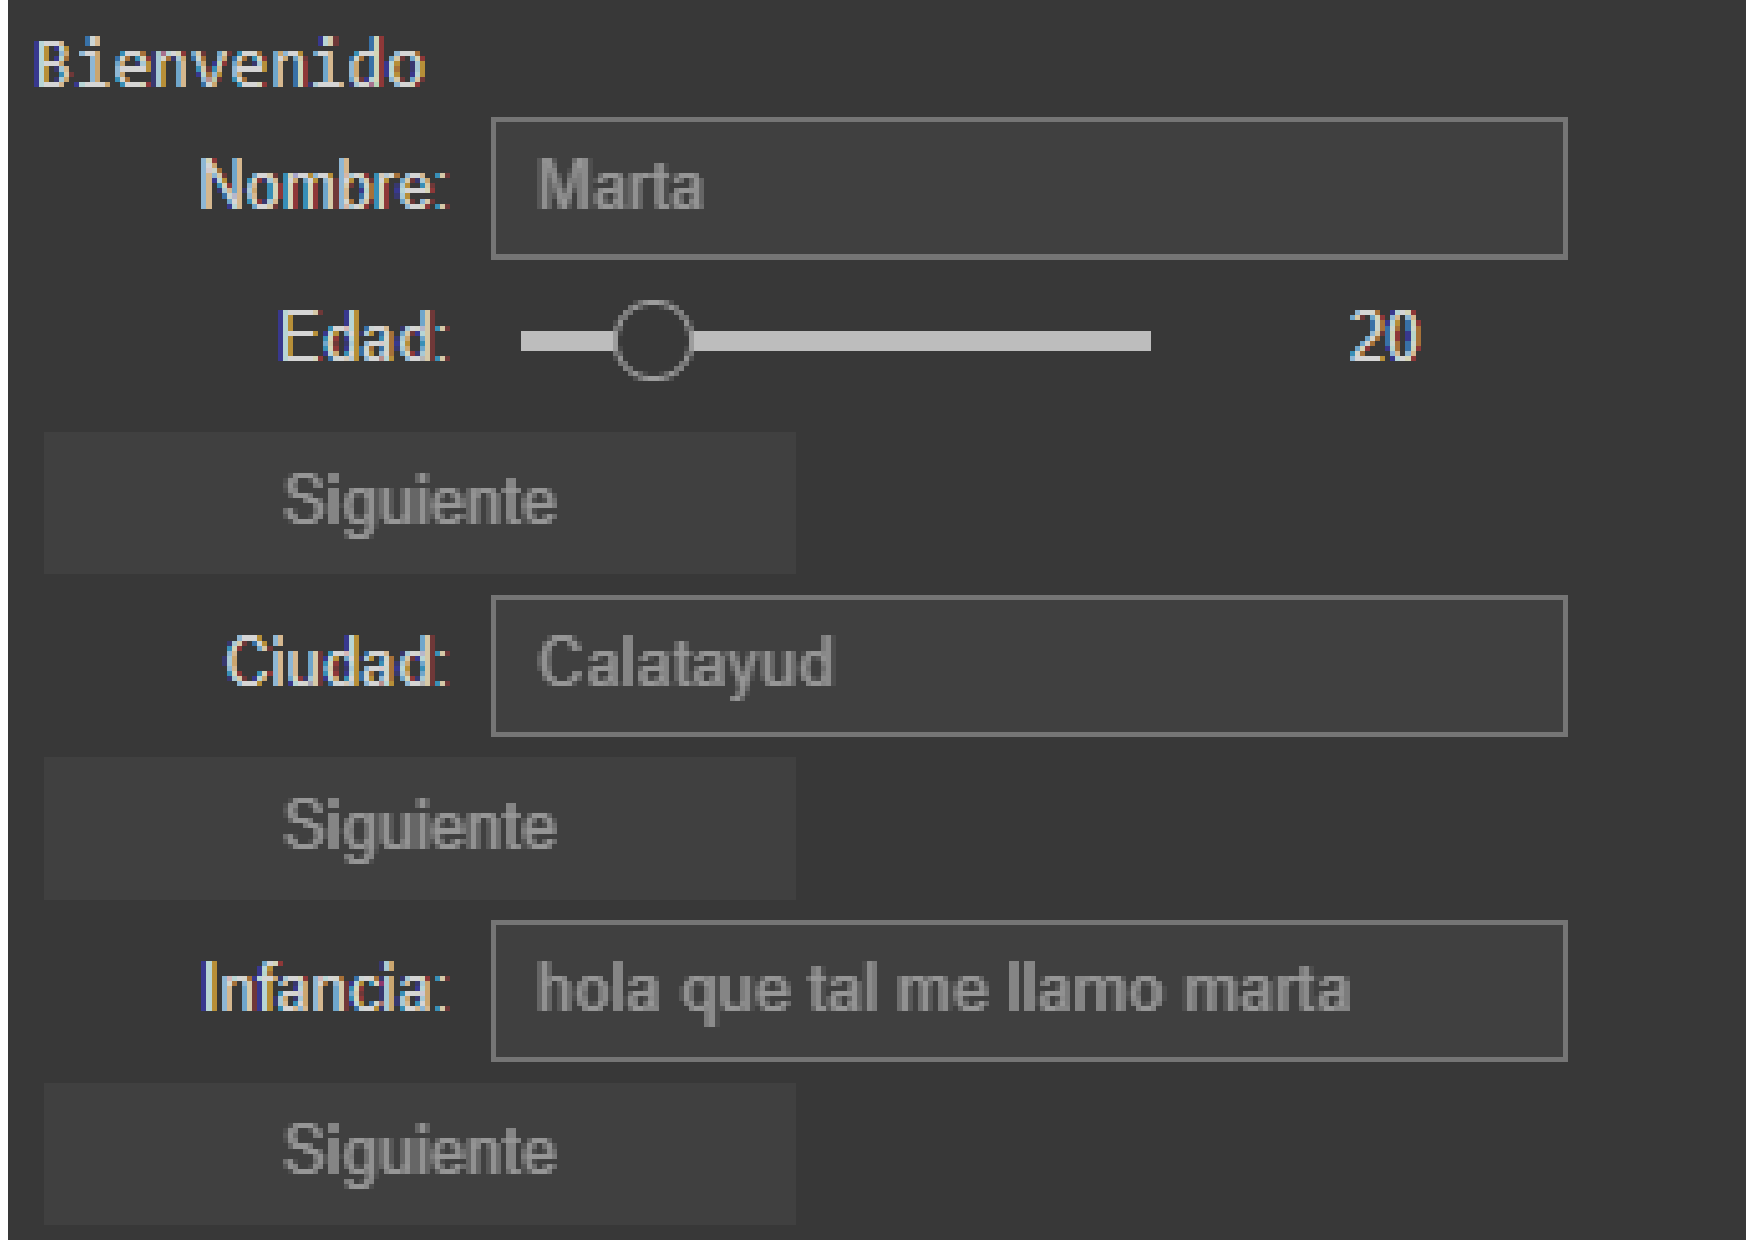
\includegraphics[width=0.5\textwidth]{Imagenes/Iwidget}
	\caption{Muestra de la interacción  con el usuario en el primer prototipo}
	\label{fig:interfazPrototipo1}
\end{figure}
Cómo se puede ver en la figura \ref{fig:interfazPrototipo1}, la interacción con el usuario se hace mediante cajas en las que se escribe la información solicitada. Una vez rellanado se envía la información al modelo para su análisis pulsando en el botón ``Siguiente'' que despliega un nuevo cuadro con la siguiente información solicitada. 

Todo este desarrollo se llevó a cabo durante los meses previos a diciembre de 2023. Fue ese mes cuando Google fortaleció la capacidad de BARD brindando habilidades más avanzadas de comprensión, razonamiento, resumen y codificación. De esta forma, paso a ser Gemini. Este cambio se oficializó en Febrero de 2024 y supuso la imposibilidad de usar BARD debido a las restricciones de uso según la localización de Gemini. Esta restricción limita el uso de la API de Gemini a una serie de regiones entre las que no se encuentra España ni ningún país de la Unión Europea.

En consecuencia, este prototipo pasó a un segundo plano y se centró el trabajo de los siguientes meses en encontrar qué API usar para el desarrollo del trabajo. Se barajaron distintas posibilidades. 

Por un lado se estudió la API de GPT por sus buenas prestaciones y características, ya presentadas en el capítulo \ref{cap:TecnologiasUtilizadas}. Sin embargo, la API es de pago y para usarla en las versiones de bajo precio o gratuito es recomendable entrenarlo lo que suponía un coste en cómputo no asumible. 

Por otro lado, se decidió estudiar distintos modelos de \textit{Hugging Face} \footnote{https://huggingface.co/} entre los que destacó Gemma. 

\section{Prototipo usando GEMMA}
Al comenzar a desasrrollar este prototipo, se trató de seguir una estructura que permitiera reutilizar todo el código posible del prototipo anterior. Para ello, se trató de desarrollar una versión de nuevo en $Google Collaborate$. Posteriormente, se estudió la alternativa de la implementación de un modelo local. En el desarrollo de este prototipo se utilizaron diferentes bibliotecas de $Hugging Face$.

\texttt{AutoTokenizer} y \texttt{AutoModelForCausalLM} son clases proporcionadas por la biblioteca $Hugging Face Transformers$ que se utilizan para cargar y trabajar con modelos de lenguaje preentrenados.

\begin{enumerate}
	\item \texttt{AutoTokenizer}: Esta clase se utiliza para cargar un tokenizador adecuado para el modelo de lenguaje preentrenado que se desea utilizar. El tokenizador se encarga de dividir el texto en unidades más pequeñas, como palabras o subpalabras, y convertirlas en vectores numéricos que el modelo de lenguaje puede entender. En nuestro contexto 
	
\begin{verbatim}
AutoTokenizer.from_pretrained(``google/gemma-7b'')
\end{verbatim}

se utiliza para cargar el tokenizador asociado al modelo de lenguaje $gemma-7b$ de Google.
	
	\item \texttt{AutoModelForCausalLM}: Esta clase se utiliza para cargar el modelo de lenguaje preentrenado que se desea utilizar. El modelo de lenguaje es responsable de generar texto basado en las entradas proporcionadas. En nuestro contexto,
\begin{verbatim}
AutoModelForCausalLM.from_pretrained(''google/gemma-7b´´)
\end{verbatim}
	
se utiliza para cargar el modelo de lenguaje "gemma-7b" de Google, que es capaz de generar texto de manera condicional, es decir, generar texto secuencialmente teniendo en cuenta el contexto anterior.
\end{enumerate}

En resumen, utilizaremos \texttt{AutoTokenizer} para cargar el tokenizador asociado al modelo de lenguaje preentrenado, y \texttt{AutoModelForCausalLM} para cargar el propio modelo. Estas clases son esenciales para preparar el modelo para su uso en la generación de texto o en otras tareas de procesamiento de lenguaje natural.

\subsection{Google Collaborate}
En primer lugar, para poder descargarnos el modelo se tiene que utilizar la biblioteca ``os'' para establecer las credenciales de autenticación de Hugging Face. Esto es necesario para acceder a modelos alojados en $Hugging Face$ y para realizar operaciones como clonar repositorios de modelos.

A continuación es necesaria la carga de la clase \textit{AutoTokenizer} y \textit{AutoModelForCausalLM} de la biblioteca \textit{Transformers} de Hugging Face para cargar un tokenizador y un modelo de lenguaje preentrenado. En este caso, el tokenizador y el modelo elegidos se cargan desde la dirección ``$google/gemma-7b$''. 

Para poder realizar todas estas instalaciones se ha de configurar el entorno de ejecución de $Google Collaborate$ de forma que se utilicen cuatro GPUs. Esto requiere seleccionar la versión ``T4 GPU'' del acelerador de hardware. Ejecutar el programa sin seleccionar esta opción impide la carga y descarga de los modelos y el programa y en consecuencia su uso. 

Una vez realizada toda esta instalación, se puede utilizar el modelo de lenguaje cargado para generar texto a partir de una entrada específica. Sin embargo, en su versión gratuita $Collaborate$ tiene limitado el uso de varios GPUs con lo que esta versión apenas pudo ser usada antes de que el entorno de ejecución limitara el uso de más de una GPU y en consecuencia, hubiera que descartar la alternativa de seguir desarrollando con $gemma-7$ en $Collaborate$.

En resumen, este código carga un modelo de lenguaje preentrenado, genera texto utilizando el modelo y realiza operaciones relacionadas con la gestión de modelos alojados en $Hugging Face$.

\subsection{Linux}
Las versiones locales de $gemma-2b$ y $gemma-7b$ en local han de ser instaladas en Linux debido a sus características. Requiere la instalación de las bibliotecas comentadas anteriormente así como de $Hugging Face$ para poder acceder a los modelos. 

En primer lugar, se optó por el modelo $gemma-2b$ pero debido a las limitaciones del mismo y a la alta exigencia de las tareas que se requieren en este proyecto, se tuvo que usar el modelo de 7 millones de parámetros. Con él, se llego a implementar una versión similar a la descrita en la sección \ref{sec:prototipoBARD} pero mediante el uso de $gemma-7b$ de $Hugging Face$. 

Se amplió este modelo, tratando de alcanzar el siguiente reto: la generación de preguntas. Para ello, se desarrolló un módulo de generación de preguntas.

El módulo en concreto aborda la tarea de generar preguntas a partir de un texto dado utilizando herramientas de procesamiento de lenguaje natural. En concreto, se centra en la biblioteca $spaCy$, una poderosa herramienta para el procesamiento avanzado del lenguaje natural que ya ha sido presentada en la sección \ref{sec:Spacy}.

La generación de preguntas comienza con la tokenización y el análisis sintáctico del texto proporcionado. Para este propósito, se utiliza el modelo preentrenado de $spaCy$ en español, denominado \textit{$``es\_core\_news\_sm''$}. Este modelo es capaz de analizar la estructura gramatical del texto y etiquetar cada token con información como el tipo de palabra (sustantivo, verbo, etc.) y la categoría gramatical.

Una vez que el texto ha sido analizado, el módulo procede a identificar los sustantivos dentro del texto. Esto se logra mediante el análisis de las etiquetas gramaticales asignadas por $spaCy$ a cada token. Cada sustantivo identificado se considera como un tema potencial para formular preguntas.

Con los sustantivos identificados, el módulo genera preguntas sobre la experiencia relacionada con cada uno de ellos. Por ejemplo, si el texto menciona la palabra es ``viaje'', el módulo formulará la pregunta ``¿Qué tal tu experiencia de viaje?''.

Para el desarrollo de la interfaz de usuario, se consideraron dos enfoques diferentes: uno utilizando el framework Flask para crear un servidor web y otro utilizando la biblioteca Tkinter para construir una interfaz gráfica de usuario (GUI) de escritorio.

Con Flask, se optó por crear un servidor web que presenta una página web con un formulario. Flask maneja las rutas y funciones asociadas, permitiendo que los usuarios ingresen información en el formulario y envíen los datos al servidor. Esto resulta en una interfaz basada en la web que puede ser accesible a través de un navegador.

Por otro lado, con Tkinter, se creó una interfaz gráfica de usuario (GUI) de escritorio. Tkinter permite crear ventanas, etiquetas y botones para construir la interfaz. En este caso, se diseñó una ventana con una etiqueta de pregunta y dos botones de opción (``Sí'' y ``No''). Esta interfaz se ejecuta localmente en la máquina del usuario y es independiente del navegador web.

Este prototipo que supone un incremento respecto al anterior también tuvo que ser descartado sin llegar a desarrollar algunas funcionalidades y módulos hasta el final, como por ejemplo la interfaz o la generación de preguntas. Este parón se debió a un problema hardware. Al instalarme Linux, y debido a restricciones de espacio en el disco duro, tuve que utilizar una partición no demasiado grande. El gran tamaño de los modelos, en concreto del modelo $gemma-7b$ ocupó gran parte del espacio de la partición. Pocas semanas después del comienzo del desarrollo de este prototipo tuvo que descartarse debido a la necesidad de ejecutarlo en Linux, acompañada de las limitaciones de espacio en mi ordenador que hicieron que no pudiera seguir desarrollandolo en ese sistema operativo. 

\section{Prototipo usando Gemini}

A lo largo de los meses se estudiaron múltiples modelos y alternativas a BARD que no resultaban lo suficientemente eficaces. Por contrario, otras sí resultaron eficaces y pese a dar lugar a pequeños prototipos no pudieron seguir desarrollándose debido a los diversos problemas que se han contado a lo largo de este capítulo. Todo este estudio, implementación de modelos y desarrollo de prototipos fallidos conlleva horas de tiempo y esfuerzo. Todo esto deriva en meses centrados en análisis de alternativas en lugar del propio desarrollo del código en sí, por lo que finalmente hubo que decantarse por la API que resultaba más eficaz y fiable y que daba mejores resultados: la API de Gemini. Como se ha comentado antes, esta alternativa se descarto en un primer momento por no estar disponible en España. Sin embargo este problema se pudo solventar fácilmente mediante el uso de VPN. 

Como ya se ha mencionado anteriormente, el segundo hito a conseguir es la construcción de una herramienta que sea capaz de analizar las respuestas, identificar la información omitida y hacer preguntas específicas para obtener la información faltante. Estas tres tareas se llevan a cabo usando la API de gemini y en concreto, el modelo $gemini-pro$. 

\subsection{Análisis de las respuestas e identificación de la información omitida}

El proceso de análisis de respuestas implica evaluar las respuestas recibidas a las preguntas planteadas durante la conversación. En nuestro caso se lleva a cabo mediante el uso del modelo y una serie de funciones que reciben como entrada la respuesta del usuario y devuelven un \textit{json} con la información asociada. Para ello, las preguntas predefinidas se almacenan en un fichero junto con una serie de campos que representan la información mínima que se quiere obtener de cada uno de ellos como se puede ver a continuación:
\begin{verbatim}
	¿Tienes hijos? : [Nombre hijos,edad hijos,recuerdos con hijos]
\end{verbatim}


El modelo, gracias a un prompt y a una llamada adecuada, se encarga de extraer la información y asociarla a cada campo, así como de indicar si hay información faltante. Pese a que se pide que la salida se devuelva como un \textit{json} esta información ha de ser parseada manualmente debido a las alucinaciones y otros fenómenos que pueden dar lugar a errores. Otro suceso que ha de ser tenido en cuenta es la posibilidad de no generación de respuesta por parte de gemini. Es por eso que hay que tener presentes en todo momento los distintos campos explicados en la sección \ref{sec:gemini}, para tener un control de qué esta ocurriendo en todo momento. 

Es por esto que se han desarrollado una serie de funciones que se encargan de transformar la respuesta en un objeto \textit{json} como se muestra a continuación. 

	\begin{verbatim}
>>>	¿Tienes hijos?
>>> Sí tengo hijos pero no estoy seguro de dónde están ahora.
     Mi hija Lucía es médico y el mayor es Juan.
>>> {'Nombre hijos': ['Lucía','Juan'], 'edad hijos': 'No
    	 Encontrado', 'recuerdos con hijos' : 'No Encontrado'}
	\end{verbatim}
	
Este prototipo también añade información adicional que haya podido obtener de la respuesta y que no se pueda asociar a los campos predefinidos. Sin embargo, estos campos son útiles para llevar un control de qué información no ha podido ser obtenida y en tal caso, generar nuevas preguntas que nos permitan obtenerla. 

 
\subsection{Generación de preguntas para obtener la información ausente}
La generación automatizada de preguntas es un componente clave del sistema diseñado. Este proceso implica la creación de nuevas preguntas dirigidas a recopilar información que no ha podido ser obtenida en las preguntas predefinidas. El proceso de generación de preguntas comienza tras la identificación de un campo al que no se ha podido asociar ningún tipo de valor o sobre el que no se ha obtenido información. En ese momento y gracias a gemini se generan una serie de preguntas asociadas asociadas a los campos que no han sido rellenados tales como las que se muestran a continuación.  

\begin{verbatim}
	>>>	'¿Cuáles son sus edades?'
	>>> '¿Cómo describe la dinámica de su familia?'
	>>> '¿Qué recuerdos tiene con sus hijos?'
\end{verbatim}
	
Estas preguntas se van lanzando al usuario hasta rellenar los campos faltantes o hasta agotar el limite de preguntas asociadas a un mismo tema que se va a hacer al usuario.

\subsection{Interfaz e interacción con el usuario}
El siguiente hito en el desarrollo del chatbot es desarrollar la interfaz que permita al usuario interactuar de una forma que resulte sencilla y práctica. Paralelamente a todo el trabajo descrito anteriormente, y durante el estudio de las diferentes alternativas de interfaces, APIs y modelos se estudio la alternativa de desarrollar la interfaz con Telegram. 

Esta opción fue encontrada al buscar alternativa a BARD o Gemma, y encontrarse diversos chatbots implementados con RASA y que adaptaban facilmente su interfaz a Telegram. Aunque la capacidad de RASA de generación de texto no cumplía los requisitos requeridos para ser considerada en este proyecto, se encontró especialmente interesante la fácil integración de chatbots con la interfaz de Telegram. 

Como se puede ver en la figura \ref{fig:ejemploRASATELEGRAM} la interfaz generada de esta forma presenta númerosas ventajas. En primer lugar, Telegram es una plataforma de mensajería ampliamente utilizada en todo el mundo, lo que garantiza un amplio alcance y accesibilidad para los usuarios y reduce la curva de aprendizaje. Además, los usuarios no sólo pueden acceder fácilmente desde su escritorio, si no también desde sus dispositivos móviles, lo que facilita su adopción y uso.

\begin{figure}
	\centering
	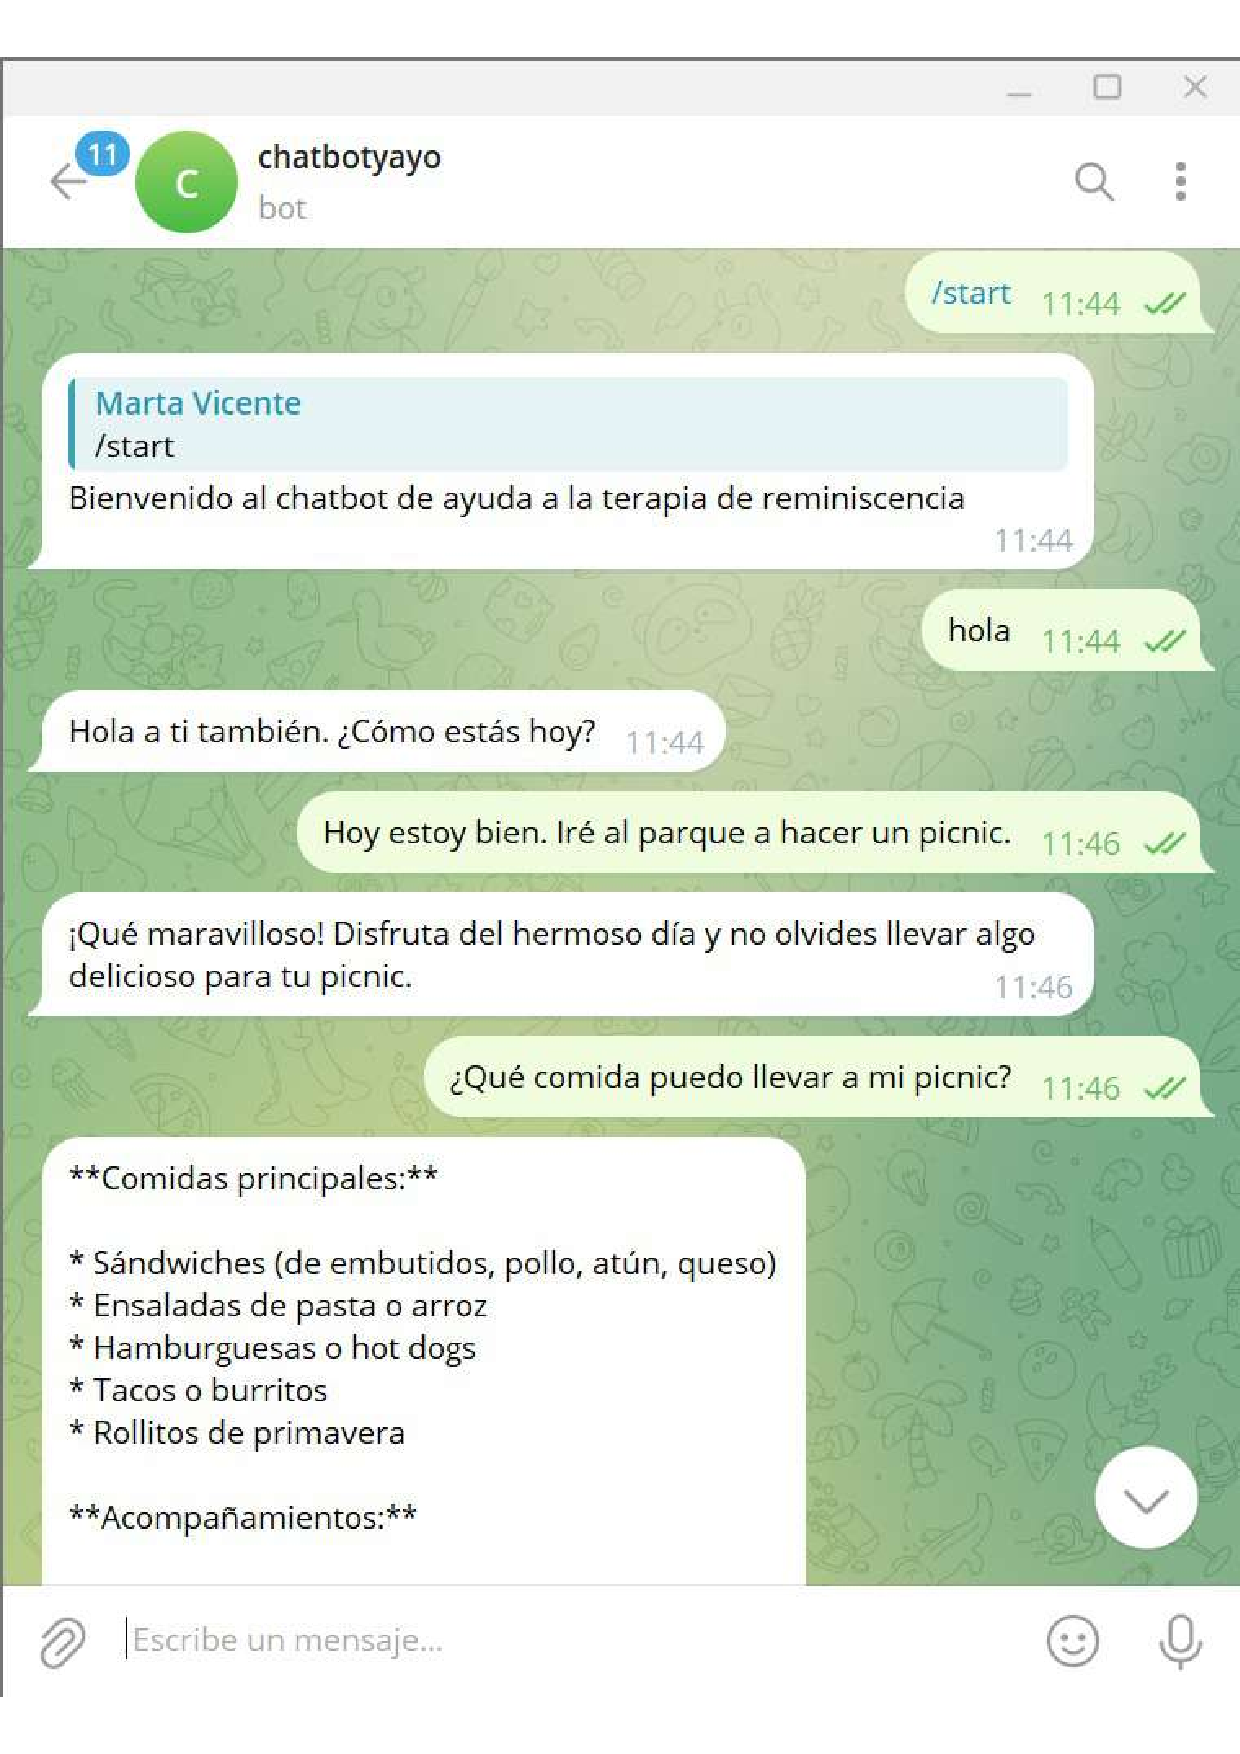
\includegraphics[width=0.5\textwidth]{Imagenes/telegram1}
	\caption{ Ejemplo de uso de BARD.}
	\label{fig:ejemploRASATELEGRAM}
\end{figure}

Esta forma de generar la interfaz implica el desarrollo de manejadores que controlen el funcionamiento según el tipo de mensaje. 

\begin{itemize}
	\item Manejadores para comandos, por ejemplo, el comando start.
	
	\item Manejadores para mensajes de texto.
	
	\item Manejadores para imagenes. 
\end{itemize}

Se utiliza la API de Telegram a través del módulo ``telebot'' para interactuar con el servicio de mensajería y gestionar los mensajes entrantes y salientes. Además, se inicia un bucle de escucha para que el bot esté constantemente activo y pueda responder a los mensajes de los usuarios en tiempo real.

Telegram también ofrece una variedad de funcionalidades integradas que pueden ser útiles para un chatbot de terapia de reminiscencia, como el envío de fotos de forma sencilla. Esto permite que la experiencia del usuario sea más rica y variada, siendo mucho más fiel a la plantilla de generación de historias de vida mencionada en la sección \ref{ssubsec:seleccionpreguntas}. Esto puede mejorar la efectividad del chatbot en la prestación de servicios de apoyo emocional.

\subsection{Clase Pregunta}
La decisión de desarrollar la interfaz del prototipo integrando Telegram y GEMINI para tener una interfaz en Telegram tuvo como consecuencia la necesidad de crear una clase Pregunta. Se crea para almacenar de manera integral toda la información asociada con una pregunta en un programa, especialmente en el contexto de la interacción con Telegram mediante textos. En versiones anteriores del desarrollo, cada vez que se requería información adicional, se realizaban preguntas y el flujo no avanzaba hasta completar estas preguntas extra o obtener la información necesaria. Al integrar esta funcionalidad con Telegram, se necesita devolver desde la función principal la información para que la interfaz pueda mostrar la pregunta, lo cual puede interrumpir el flujo original del código. Esta integración conlleva a una refactorización que dio lugar a la creación de la clase ``Pregunta''.

La clase ``Pregunta'' encapsula una pregunta con su enunciado, respuesta, campos asociados y preguntas adicionales relacionadas. Su objetivo principal es proporcionar una estructura organizada para manejar la información de una pregunta específica y sus detalles. Permite actualizar la respuesta principal, indicar el estado de los campos (respondidos o no respondidos), agregar preguntas adicionales relacionadas y gestionar las respuestas a estas preguntas secundarias.

Además, la clase ``Pregunta'' ofrece métodos para actualizar la respuesta, marcar campos como respondidos, agregar preguntas adicionales, gestionar las respuestas a estas preguntas secundarias y obtener una representación textual de la instancia de la clase.

\subsection{Telegram}
\label{sec:Telegram}
La integración del prototipo con \textit{Telegram} requiere importar la biblioteca $telebot$ que es la que permite la comunicación entre el modelo y la interfaz. 

Para conectar Telegram con el chatbot desarrollado a través de la API de Gemini, fue necesario obtener un token de Telegram. Es importante mencionar que este paso forma parte de la configuración inicial y no requiere intervención por parte del usuario final durante la puesta en marcha.

Este token se obtuvo a través del usuario de telegram $\makeatletter @ BotFather$ y con el comando $\backslash newbot$ y $\backslash token$. Una vez con el token se creo el \textit{chatbotyayo} con nombre de usuario $\makeatletter @ mavice07\_bot$. Para comenzar a interactuar con \textit{chatbotyayo} basta con buscar ese usuario en Telegram y enviar el comando $\backslash start$. 

Una vez obtenido el token y finalizadas todas las configuraciones se implementa la lógica del sistema. Se definen tres manejadores de mensajes:
	\begin{itemize}
		\item El manejador $cmd\_start()$ se activa únicamente cuando un usuario envía el comando $\backslash start$ al bot. Este manejador inicia la lógica del bot al cargar las preguntas utilizando la función $cargar\_preguntas()$ del módulo $tfg$ y envía un mensaje de bienvenida al usuario.
		
		\item El manejador $bot\_mensajes\_text()$ se activa cuando un usuario envía un mensaje de texto al bot. Si el mensaje comienza con "$\backslash$", se envía un mensaje de error indicando que el comando no está disponible. Si es un mensaje de texto estándar, se llama a la función $siguientePregunta()$ del módulo $tfg$ y se analiza el mensaje como respuesta al último mensaje enviado por el bot. De esta forma se procesa la respuesta del usuario y se genera una respuesta apropiada.
		
		\item El manejador $photo()$ se activa cuando un usuario envía una foto al bot. El bot descarga la foto, la guarda en el sistema de archivos y llama a la función $analizador\_imagenes()$ del módulo $imagenes$ para analizar la imagen y generar una respuesta apropiada.
	\end{itemize}
	
Finalmente, se inicia el bucle de escucha del bot $bot.infinity\_polling()$ para que esté constantemente esperando y respondiendo a los mensajes de los usuarios.


\subsection{Extracción de información a partir de imagenes}
\label{sec:imagenes}
La api de Gemini tiene muchas funcionalidades que permiten del chatbot una herramienta completa. En concreto, gracias a la interfaz elegida y al modelo \textit{gemini-pro-vision} se ha implementado una funcionalidad extra respecto a las que estaban planteadas originalmente. Esta funcionalidad es la extracción de información a partir de imagenes. En cualquier momento, el usuario puede adjuntar una foto. El programa se encarga de analizar la fotografía y a partir de ella hacer preguntas que permitan extraer más información que la obtenida únicamente con las preguntas.

Mediante el reconocimiento y clasificación de objetos, personas y lugares en imágenes, el procesamiento de imagenes puede identificar elementos significativos que pueden evocar recuerdos en los pacientes. 

El análisis de imágenes también puede proporcionar contexto y significado a las experiencias pasadas. Examinar el contenido visual de las fotografías, puede ayudar a contextualizar recuerdos específicos, facilitando así la conversación y la narración de historias durante las sesiones de terapia. La selección cuidadosa de imágenes personalizadas para cada paciente puede estimular recuerdos y promover interacciones significativas. 

\begin{figure}[h]
	\centering
	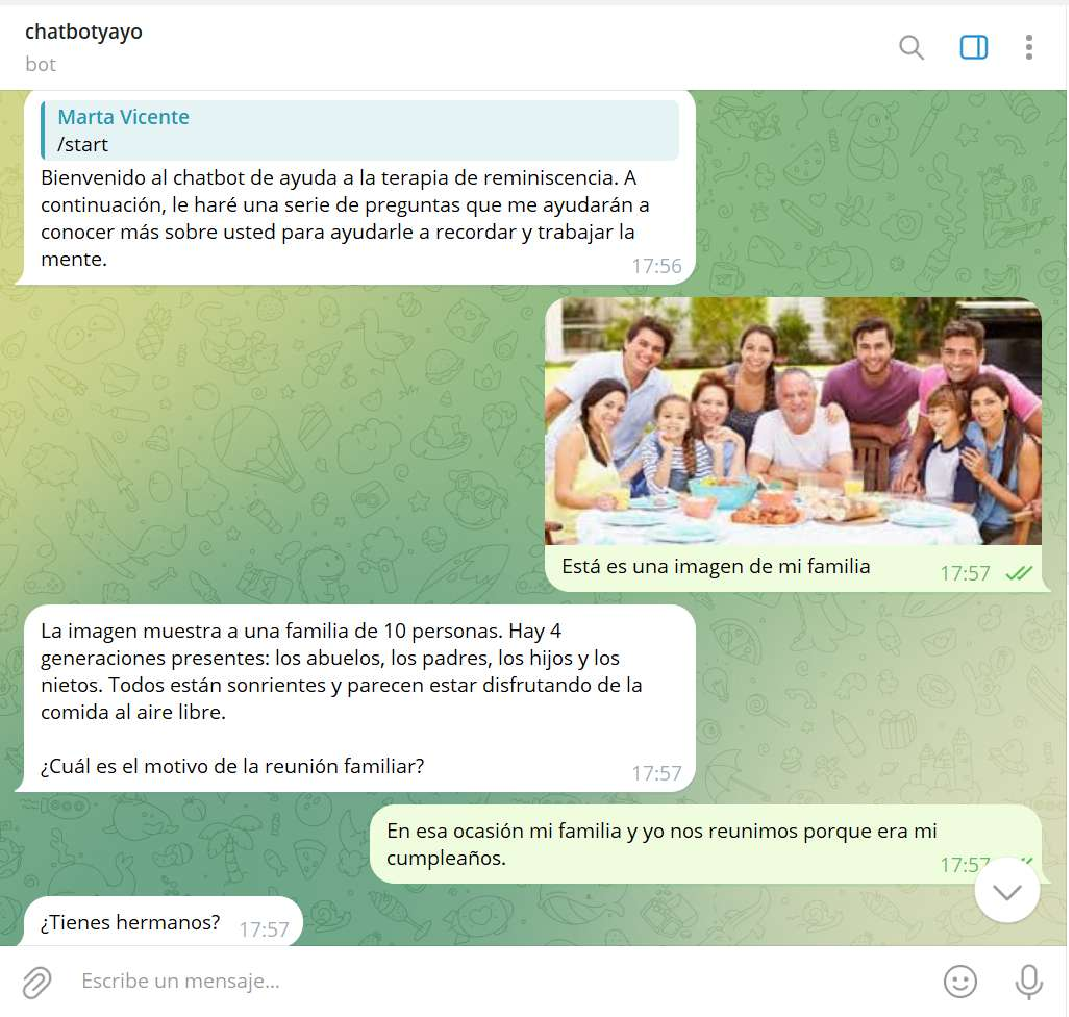
\includegraphics[width=0.9\textwidth]{Imagenes/extracInfoImag}
	\caption{Ejemplo de extracción de información a partir de imagenes}
\end{figure}

